\begin{definition}
    Пусть имеется дифференциальное уравнение вида 
    \[
    \dot{x} = f(x)\eqno{(*)}
    \]
    Функцию $\phi(x)$, не являющуюся тождественной константой, назовем \textbf{первым интегралом} $(*)$, если $\phi(x(t)) = c(x(t_0))$, т.е. $\phi$ сохраняет свое значение на любом решении.
\end{definition}

Все системы сил делятся на интегрируемые и неинтегрируемые. Системы первого типа сводятся к гармоническому осциллятору.

\begin{definition}
    Две системы сил называются \textbf{эквивалентными}, если у них равны главные векторы и моменты сил относительно любого полюса.
\end{definition}

Аналогично случаю для \hyperlink{K_pole_shift}{кинетического момента}, можно получить формулу переноса полюса для момента сил системы:
\[
    \begin{cases}
        \vec{M}_A = \sum \vec{r}_{A_i} \times \vec{F}_i\\
        \vec{M}_B = \sum \vec{r}_{B_i} \times \vec{F}_i\\
    \end{cases} \Longrightarrow \vec{M}_B = \vec{M}_A + \vec{F} \times \vec{AB}
    \]
Тогда
\begin{enumerate}
    \item $\vec{F}$ --- главный вектор сил --- 1 статистический инвариант.
    \item $\left| \dfrac{\vec{M}_B \cdot \vec{F}}{|\vec{F}|}\right| = \left| \dfrac{\vec{M}_A \cdot \vec{F}}{|\vec{F}|}\right| = M_{min}$ --- 2 статистический инвариант.
    \item Пусть $|M_O| = M_{min}$, каково геометрическое место таких точек О?\\
    $\vec{M}_O~ || ~\vec{F}$ $\Longrightarrow$ ось минимальных моментов.
\end{enumerate}

Рассмотрим случаи.
\begin{figure}[!h]
    \centering
    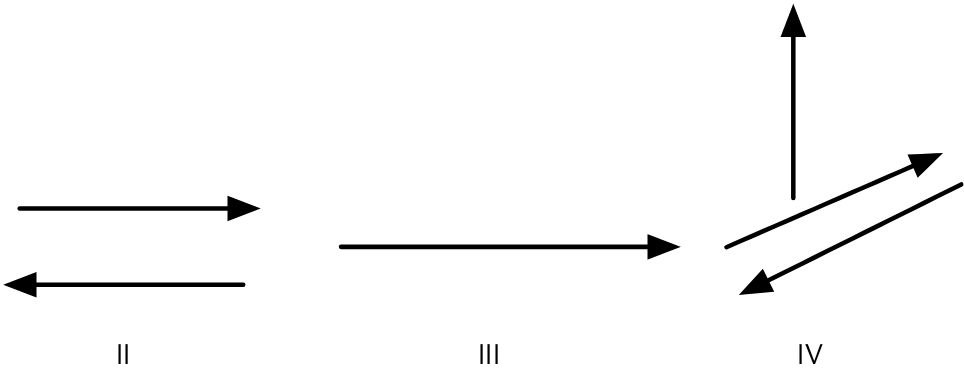
\includegraphics[width=0.75\linewidth]{images/лекция_7_1.jpeg}
\end{figure}
\begin{enumerate}
    \item[(I)] $F = 0$, $M_{min} = 0$\\
    Система сил уравновешена.
    \item[(II)] $F = 0$, $M_{min} \neq 0$\\
    Пара сил.
    \item[(III)] $F \neq 0$, $M_{min} = 0$
    Только в этом случае можно говорить о замене на равнодействующую.
    \item [(IV)] $F \neq 0$, $M_{min} \neq 0$\\
    Это динамический винт.
\end{enumerate}




\subsection{Основные теоремы динамики в неинерциальных системах отсчета}

\begin{wrapfigure}{l}{0.5\textwidth}
  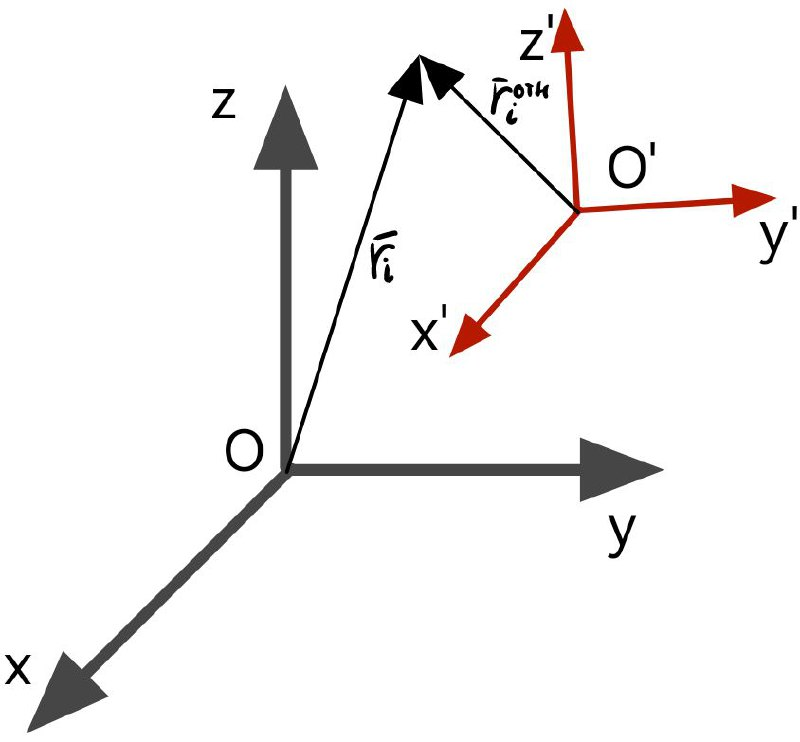
\includegraphics[width=0.8\linewidth]{images/лекция_7_2.jpeg}
\end{wrapfigure}
Рассмотрим две системы отсчета: $O_{xyz}$ --- инерциальная и $O'_{x'y'z'}$ --- неинерциальная.\\

В неинерциальной системе отсчета уравнения движения точки имеют вид:
\[
\vec{w}_i^{\text{абс}} = \vec{w}_i^{\text{пер}} + \vec{w}_i^{\text{отн}} + \vec{w}_i^{\text{кор}},
\]
где
\[
\vec{w}_i^{\text{пер}} = \vec{w}_{O'} + \vec{\varepsilon} \times \vec{r}_i^{\text{отн}} + \vec{\omega} \times (\vec{\omega} \times \vec{r}_i^\text{отн}), \ \vec{w}_i^{\text{кор}} = 2\vec{\omega} \times \vec{v}_i^{\text{отн}}
\]
$\vec{w}_i^{\text{пер}}$ --- \textbf{переносное ускорение}, $\vec{w}_i^{\text{кор}}$ --- \textbf{кориолисово ускорение}.\\

Перепишем основные теоремы в случае неинерциальных систем. Доказываются они по аналогии с инерциальным случаем.\\

\begin{theorem}[Теорема об изменении импульса]
    Пусть $\vec{J}^\text{пер} = - \sum m_i \vec{w}_i^\text{пер} = -m \vec{w}_C^\text{пер}$ --- ,\textbf{переносная сила инерции} $\vec{J}^\text{кор} = - \sum m_i \vec{w}_i^\text{кор} = -m \vec{w}_C^\text{кор}$ --- \textbf{кориолисова сила инерции}. Тогда импульс системы меняется по закону
    \[
    \dfrac{d \vec{P}^{\text{отн}}}{d t} = \vec{F}^{out} + \vec{J}^\text{пер} + \vec{J}^\text{кор}
    \]
\end{theorem}

\begin{theorem}[Теорема об изменении кинетического момента]
    Пусть $C$ --- центр масс тела, $A$ --- некоторый его полюс. \textbf{Переносной} и \textbf{кориолисов моменты сил} определяются как $\vec{M}_A^\text{пер} = - \sum \vec{r}_{A_i} \times m_i\vec{w_i}^\text{пер}$ и $\vec{M}_A^\text{кор} = - \sum \vec{r}_{A_i} \times m_i\vec{w_i}^\text{кор}$ соответственно. Тогда кинетический момент относительно полюса $A$ изменяется по закону
    \[
    \dfrac{d \vec{K}_A^\text{отн}}{d t} = \vec{M}_A^{out} + \vec{M}_A^\text{пер} + \vec{M}_A^\text{кор} + m\vec{v}_C^\text{отн} \times \vec{v}_A^\text{отн}
    \]
\end{theorem}

\begin{figure}[!h]
        \centering
        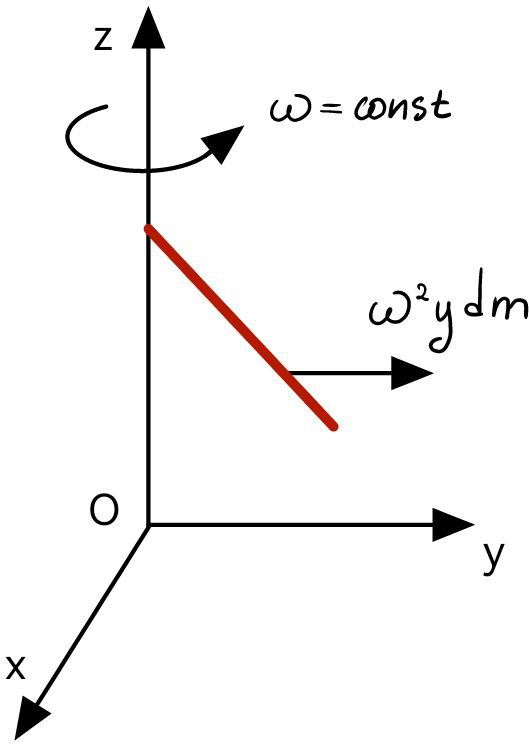
\includegraphics[width=0.25\linewidth]{images/лекция_7_3.jpeg}
    \end{figure}
\begin{example}
    Найдем переносные силу и момент сил для вращающегося с постоянной угловой скоростью стержня, показанного на рисунке.
\end{example}

\[
\vec{F}_i^\text{пер} = \int\limits_\text{по стержню} \omega^2y~d m \cdot \begin{pmatrix}
    0\\
    1\\
    0
\end{pmatrix}
\]
\[
\vec{M}_A^\text{пер} = \int\limits_\text{по стержню} \vec{r}~dm \cdot \begin{pmatrix}
    0\\
    1\\
    0
\end{pmatrix}\omega^2y~d m
\]

\begin{theorem}[Теорема об изменении кинетической энергии]
    Кинетическая энергия меняется по закону
    \[
    \dfrac{d \vec{T}^{\text{отн}}}{d t} = N^{out} + N^{in} + N^\text{пер}
    \]
    или
    \[
    dT^\text{отн} = \delta A^{out} + \delta A^{in} + \delta A^\text{пер}
    \]
\end{theorem}
В последней теореме слагаемое, отвечающее за мощность кориолисовых сил, обращается в ноль:
\[
N^\text{кор} = \sum \vec{J}_i^\text{кор} \cdot \vec{v}_i^\text{отн} = -2\sum m_i \cdot (\vec{\omega} \times \vec{v}_i^\text{отн}) \vec{v}_i^\text{отн} = 0
\]

\begin{definition}
    Силы с нулевой мощностью называются \textbf{гироскопическими}. Так, кориолисовы силы являются гироскопическими.
\end{definition}

\begin{note}
    В осях Кенига вид теорем упрощается:
    \[
    \vec{P}^\text{отн} = 0
    \]
    \[
    \dfrac{d \vec{K}_C^{\text{отн}}}{d t} = \vec{M}_C^{out}
    \]
    \[
    \dfrac{d T^{\text{отн}}}{d t} = N^{out} + N^{in}
    \]
\end{note}

\subsection{Динамика реактивного движения}
Рассмотрим теперь ситуацию, когда в процессе движения масса тела может меняться. Причем считаем, что за малый промежуток времени $\Delta t$ масса изменяется мало. Тогда на точку также будут действовать \textbf{реактивные} силы.\\

Рассмотрим точку с массой m c изначальной скоростью $\vec{v}$ в два момента времени: $t$ и $t + \Delta t$. За $\Delta t$ к точке добавилась масса $\Delta m_1$, двигавшаяся до этого скорость $\vec{u_1}$; точку покинула масса $\Delta m_2$ со скоростью $\vec{u_2}$. Количество движения системы в эти моменты времени:
\[
\vec{P}(t) = m\vec{v} + \Delta m_1 \vec{u_1}
\]
\[
\vec{P}(t + \Delta t) = (m + \Delta m_1 - \Delta m_2)(\vec{v} + \Delta \vec{v}) + \Delta m_2 \vec{u_2}
\]
Тогда получим, что
\[
\dfrac{d \vec{P}}{d t} = \lim\limits_{\Delta t \longrightarrow 0} \dfrac{\vec{P}(t + \Delta t) - \vec{P}(t)}{\Delta t} = \vec{F}^{out}
\]
или
\[
m\dfrac{d \vec{v}}{d t} + \dfrac{d m_1}{d t}(\vec{v} - \vec{u_1}) - \dfrac{d m_2}{dt}(\vec{v} - \vec{u_2}) = \vec{F}^{out}
\]
Здесь \textbf{реактивная сила} $\vec{R} = \dfrac{d m_1}{d t}(\vec{u_1} - \vec{v}) - \dfrac{d m_2}{dt}(\vec{u_2} - \vec{v})$.


\subsection{Динамика точки в центральном поле}
\subsubsection{Движение точки в поле неподвижного центра}
\begin{wrapfigure}{r}{0.2\textwidth}
  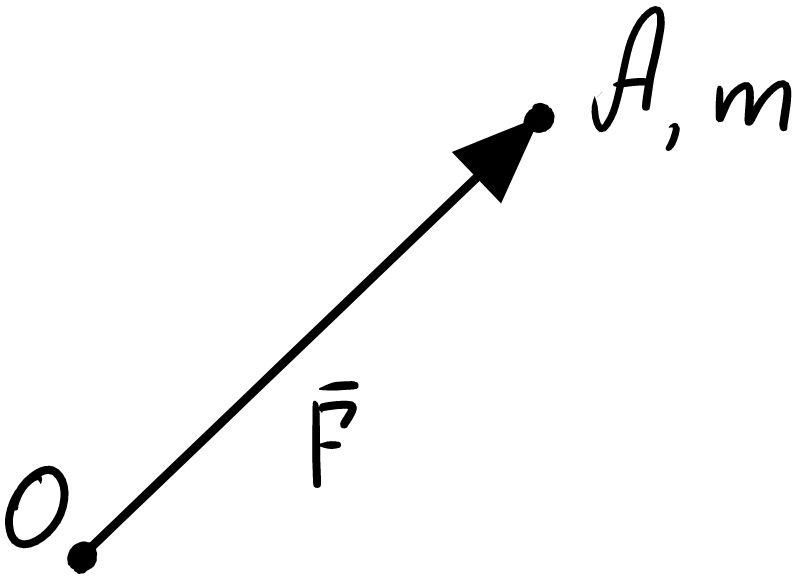
\includegraphics[width=0.8\linewidth]{images/лекция_7_4.jpeg}
\end{wrapfigure}
Рассмотрим точку $A$ массой m, которая движется под действием \textbf{центральной} силы $\vec{F}$, т.е. в любой момент времени $\vec{OA}~||~\vec{F}$, где $O$ --- силовой центр.\\

Т.к. момент сил относительно $O$ $\vec{M}_O = \vec{OA} \times \vec{F} = 0$, то по \hyperlink{theorem_delta_K}{теореме об изменении кинетического момента} кинетический момент относительно $O$ не меняется со временем, значит, движение плоское ($\vec{K}_O$ перпендикулярен плоскости).\\

Перейдем к полярным координатам. Тогда
\[
\vec{v} = \dot{\rho}\vec{e}_\rho + \rho \dot{\phi} \vec{e}_\phi \ \Longrightarrow  \ v^2 = \dot{\rho}^2 + (\rho \dot{\phi})^2
\]
Здесь $\vec{e}_\rho$ и $\vec{e}_\phi$ --- единичные векторы.
\[
w_\rho = \ddot{\rho} - \rho\dot{\phi}^2 \tab w_\phi = \dfrac{1}{\rho}\dfrac{d}{dt}(\rho^2\dot{\phi})
\]
Тогда с помощью второго закона Ньютона получаем
\[
\begin{cases}
    m(\ddot{\rho} - \rho\dot{\phi}^2) = F\\
    mw_\phi = 0
\end{cases}
\]
Из второго равенства следует \textbf{второй закон Кеплера}:
\[
\rho^2\dot{\phi} = c = 2 \dot{S},
\]
где $\vec{c} = \vec{r} \times \vec{v}$ --- кинетический момент единичной массы, $S$ --- площадь, заметаемая радиус-вектором $\vec{r}$.

\subsubsection{Уравнение Бине}
Рассмотрим случай, когда сила зависит только от расстояния до выбранной точки, т.е.
\[
m(\ddot{\rho} - \rho\dot{\phi}^2) = F(r)
\]
Это случай \textbf{центрально-симметричного} поля. Используя второй закон Кеплера и \textbf{замену Бине} $\rho = \dfrac{1}{u}$, можем исключить время из уравнения выше (считаем, что штрих --- это производная по $\phi$):
\[
\dot{\rho} = \dfrac{d \rho}{d t} = \dfrac{d \dfrac{1}{u}}{d \phi}\dot{\phi} = -\dfrac{1}{u^2}u'\dot{\phi} = - \dfrac{1}{u^2}u'\cdot cu^2 = -c u'
\]
\[
\ddot{\rho} = \dfrac{d(-cu')}{d \phi}\dot{\phi} = -c^2u^2u''
\]
\[
    -c^2u^2u'' - c^2u^3 = \dfrac{F\left(\dfrac{1}{u}\right)}{m}
\]
Итого, \textbf{уравнение Бине}:
\[
u'' + u = -\dfrac{F\left(\dfrac{1}{u}\right)}{mc^2u^2}
\]
\subsubsection{Ньютоновское поле}
В случае ньютоновского поля
\[
F = - \gamma \dfrac{Mm}{r^2} = -\dfrac{\alpha m}{r^2}
\]

Уравнение Бине принимает вид
\[
u'' + u = \dfrac{\alpha}{c^2}
\]
Решение будет иметь вид $u(\phi) = A \cos(\phi + \phi_0) + \dfrac{\alpha}{c^2}$. Переобозначим $p = \dfrac{c^2}{\alpha}$ --- \textbf{фокальный параметр}, $e = Ap$ --- \textbf{эксцентриситет}, тогда уравнение конического сечения:
\[
r = \dfrac{p}{1 + e \cos{(\phi - \phi_0)}}
\]